\documentclass[a4paper]{assignment}

\usepackage[left=3cm, right=2.5cm]{geometry} % Hier die Ränder definieren

\usepackage [latin1]{inputenc}


\usepackage[pdftex]{graphicx}
%%%%% Path for Pictures %%%%%%
\graphicspath{ {./Pictures} }
\usepackage{subfigure} 
\usepackage[backend=biber,style=numeric,url=true]{biblatex} % für Quellenangaben und Bibliotheken
\usepackage[]{hyperref} % für hyperlinks
\usepackage{array} % für die Tabelle
\addbibresource{quellen.bib}  % Add your .bib file here

% Paket für die Baumdiagramdarstellung
\usepackage{tikz}
\usetikzlibrary{trees}

% https://chatgpt.com/c/68191c8e-8760-8002-843b-e82091955567
\usepackage{booktabs} % für schönere Tabellenlinien
\usepackage{amsmath}  % für mathematische Symbole wie \left[ \right]
\usepackage{amssymb}

%%%% Packet um die Farbe von text zu ändern %%%%
%\textcolor{red}{text}
%\definecolor{mygreen}{RGB}{0,150,0}
%\textcolor{mygreen}{Dies ist grüner Text mit eigener Farbe.}
%{\color{blue}
%Dies ist ein ganzer Absatz in Blau.
%}
\usepackage{xcolor}

%%%%% draws layout frames %%%%%
%\usepackage{showframe}

%%%%% Multiple Columns %%%%%
% see: https://www.overleaf.com/learn/latex/Multiple_columns
\usepackage{multicol}


% Text block indentation
%\lipsum[1]
%\begin{addmargin}[1em]{2em}% 1em left, 2em right
%\lipsum[2]
%\end{addmargin}
%\lipsum[3]
\usepackage{scrextend}



\hypersetup{
    colorlinks=true,
    linkcolor=blue,
    filecolor=magenta,      
    urlcolor=cyan,
    pdftitle={Overleaf Example},
    pdfpagemode=FullScreen,
    }
    

%%% Code-Block design
%%% Benutzung mit: 
%%%%% \lstinputlisting[language=Scala]{./Code/Hashtable.scala} %%% für datein
%%%%% \begin{lstlisting}[language=Scala] %%% für \begin und \end
% https://www.overleaf.com/learn/latex/Code_listing
\usepackage{listings}

\definecolor{codegreen}{rgb}{0,0.6,0}
\definecolor{codegray}{rgb}{0.5,0.5,0.5}
\definecolor{codepurple}{rgb}{0.58,0,0.82}
\definecolor{backcolour}{rgb}{0.95,0.95,0.92}

\lstdefinestyle{mystyle}{
    backgroundcolor=\color{backcolour},   
    commentstyle=\color{codegreen},
    keywordstyle=\color{magenta},
    numberstyle=\tiny\color{codegray},
    stringstyle=\color{codepurple},
    basicstyle=\ttfamily\footnotesize,
    breakatwhitespace=false,         
    breaklines=true,                 
    captionpos=b,                    
    keepspaces=true,                 
    numbers=left,                    
    numbersep=5pt,                  
    showspaces=false,                
    showstringspaces=false,
    showtabs=false,                  
    tabsize=2
}
\lstset{style=mystyle}




\begin{document}

% Aufgabe 1 Binäre Suchbäume)
\begin{problemlist}

\pbitem{Induktion und binäre Bäume} \\
Ein binärer Baum heißt vollständig, falls jeder Knoten entweder null oder zwei Kinder besitzt.
\begin{enumerate}

\item Zeichnen Sie einen binären Suchbaum, der vollständig ist, und einen binären Suchbaum, der nicht vollständig ist.

\begin{answer}
\begin{itemize}
	\item Balancierter vollständiger BTS:
\end{itemize}
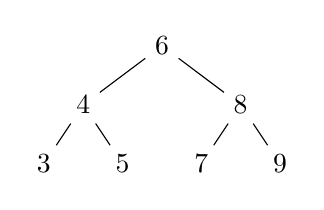
\begin{tikzpicture}[scale=0.5,
  level 1/.style={sibling distance=40mm},
  level 2/.style={sibling distance=20mm}]
\node{6}
	child{node{4}
		child{node{3}}
		child{node{5}}}
	child{node{8}
		child{node{7}}
		child{node{9}}};
\end{tikzpicture}

\begin{itemize}
	\item Unvollständiger BTS:
\end{itemize}

\begin{tikzpicture}[scale=0.5,
  level 1/.style={sibling distance=40mm},
  level 2/.style={sibling distance=20mm}]
\node{6}
	child{node{4}
		child{node{3}
			child{node{1}}
			child[missing]}
		child{node{5}}}
	child{node{8}
		child{node{7}}
		child{node{9}}};
\end{tikzpicture}

\end{answer}

\item Beweisen Sie durch eine geeignete Induktion: In jedem vollständigen binären Suchbaum ist die Anzahl der Blätter genau um eins größer als die Anzahl der inneren Knoten.

\begin{answer}
\begin{itemize}
	\item n jedem vollständigem BTS gilt: jeder Knoten n hat 0 oder genau 2 Kindknoten. 
    \item innerer Knoten: jeder Knoten v gilt als innerer Knoten gdw. v min. 1 Kindknoten hat.
    \item Blätter Knoten: Jeder Knoten v gilt als Blatt, wenn v keine Kinderknoten hat.
\end{itemize}

\textbf{Annahme:} In jedem vollständigen binären Suchbaum ist die Anzahl der Blätter genau um eins größer als die Anzahl der inneren Knoten. \\

base-case BTS mit einem inneren Knoten (root): \\
Angenommen der BTS erfüllt die Bedingungen eines vollständigen BTS und die Werte der Knoten spielen keine Rolle, dann muss gelten:  \\
$num_{\text{Blätter}}=num_{\text{innerer Knoten}}+1$


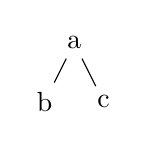
\begin{tikzpicture}[scale=0.5]
\node{a}
	child{node{b}}
	child{node{c}};
\end{tikzpicture}

Da die Werte in diesem Fall unerheblich sind, gilt die Zeichnung für einen vollständingen BTS mit einem inneren Knoten: \\
\begin{itemize}
	\item $num_{\text{innerer Knoten}}=a \text{ } num_{\text{innere Knoten}}=1$ 
	\item $num_{\text{Blätter}}=b,c \text{ } num_{\text{Blätter}}=2$ 
\end{itemize}

Die Anahme gilt im base-case. \\

\textbf{I.S:} Wenn die Annahme bei n inneren Knoten gilt, gilt sie auch $n+1$ inneren Knoten. 
Ein vollständiger BTS mit n inneren Knoten erfüllt die Gleichung:  \\
$num_{\text{Blätter}} = num_{\text{innerer Knoten}} + 1$ \\
Wenn es einen inneren Knoten zusätzlich geben soll, wird ein Blattknoten zu diesem Knoten und bekommt nach der Definition von vollständigen BTS 2 neue Kindknoten, da:

\begin{enumerate}
	\item nur 1 Kind Widerspruch mit Definition von vollständigen BTS.
	\item 0 Kindknoten, dann bleibt $num_{\text{innerer Knoten}}$ gleich, da das Blatt nicht zum Inneren Knoten werden konnte.
\end{enumerate}

\end{answer}


\item Formulieren Sie eine ähnliche Aussage für allgemeine binäre Suchbäume und beweisen Sie sie.
\end{enumerate}

\newpage
\section*{Problem 1: Kryptographische Hashfunktionen und Blockchain}

\subsection*{a) Kryptographische Hashfunktionen in Scala}

Welche kryptographischen Hashfunktionen sind in Scala implementiert?  
Wie kann man sie verwenden?


\subsubsection*{Lösung: Non-cryptographic hashfunctions}

Scala3 hat keine eigene Kryptographische Hashfunktion Implementiert (jedenfalls habe ich nichts gefunden). \\

In Scala hat man die Möglichkeit interne Hashfunktionen zu benutzten wie z.B. mit hashCode() methode\cite{hashCode}:
\begin{lstlisting}[language=Scala]
scala> val result = "hello".hashCode()
val result: Int = 99162322
\end{lstlisting}
Dies dient aber nicht der Kryptographischen Verschlüsselung von Werten, da es hierbei zu viele Kollisionen kommt, eher ist es zur Kontrolle von Werten gedacht.\\

Eine weitere Möglichkeit ist es über eine zusätzliche Scala Library zusätzliche Hashfunktionen zu benutzen: \textit{scala.util.hashing.Hashing} \cite{scala.util}\\

\lstinputlisting[language=Scala]{./Code/Scalatest.scala}

\begin{verbatim}
Output: 69490486
\end{verbatim}

\subsubsection*{MurmurHash3}

Oder auch eine Implementierung von MurmurHash3 von Rex Kerr. Auch dieser ist aber ein \textit{non-cryptographic hashing algorithm} \cite{murmurhash3}

\lstinputlisting[language=Scala]{./Code/murmurHash3.scala}

\begin{verbatim}
Output: -608680269
\end{verbatim}

\subsubsection*{Kryptographische Hashfunktionen}

Um Kryptographische Hashfunktionen in Scala zu benutzen, müssen wir auf Bibliotheken von Java zurückgreifen. Um dies zu tun, Importieren wir z.B.:\textit{java.security.MessageDigest} - für die Nutzung von SHA-256, MD5 oder auch SHA-1.\cite{sha-256}

\begin{lstlisting}[language=Scala]
import java.security.MessageDigest
\end{lstlisting}

Um z.B.: SHA-256 zu verwenden, müssen wir die vorgefertigten Methoden, getInstance(), digest(), benutzen

\begin{lstlisting}[language=Scala]
import java.security.MessageDigest


@main def run(): Unit =

  val message = "Hello World"
  val sha256 = MessageDigest.getInstance("SHA-256")
  val hashWert = sha256.digest(message.getBytes("UTF-8"))

  println(hashWert)
\end{lstlisting}

\begin{verbatim}
Output: [B@45820e51
\end{verbatim}

\begin{itemize}
\item MessageDigest - ruft das Objekt auf
\item getInstance() - Returns a MessageDigest object that implements the specified digest algorithm.
\item digest - Performs a final update on the digest using the specified array of bytes, then completes the digest computation.
\end{itemize}

Da wir bei \textit{println(hashWert)} eine Standard-toString-Ausgabe von einem Java-Array erhalten( also in Bytes ), müssen wir die Ausgabe noch einmal in Hex-Zahlen umwandeln:

\lstinputlisting[language=Scala]{./Code/SHA-256.scala}
\begin{verbatim}
Output: a591a6d40bf420404a011733cfb7b190d62c65bf0bcda32b57b277d9ad9f146e
\end{verbatim}

\vspace{1em}

\subsection*{b) Verkettete Liste mit Hashreferenzen}

Implementieren Sie in \texttt{Scala} eine einfach verkettete Liste mit Hashreferenzen.  
In den Knoten der einfach verketteten Liste sollen \texttt{String}-Objekte gespeichert werden.  
Verwenden Sie dazu eine kryptographische Hashfunktion wie in Teil (a).

\vspace{1em}

\subsection*{c) Nonce und Hash mit Nullen am Ende}

Fügen Sie zu den Knoten Ihrer einfach verketteten Liste jeweils ein \emph{Nonce} hinzu,  
und stellen Sie sicher, dass die Hashwerte in den Referenzen alle mit acht Nullen (in der Binärdarstellung) enden.  

Wie viele Versuche sind dazu im Durchschnitt nötig?

\newpage

\newpage
\pbitem{Binäre Suchbäume}
\begin{enumerate}
\item Angenommen, wir haben einen binären Suchbaum T , welcher die Zahlen von
1 bis 1000 als Schlüssel speichert. Wir suchen in T nach dem Schlüssel 363.
Bestimmen Sie für jede der folgenden Schlüsselfolgen, ob sie als Folge der
Einträge auf dem Suchpfad nach 363 auftreten kann. Begründen Sie jeweils
Ihre Antwort.


\begin{enumerate}
\item \textbf{2, 252, 401, 398, 330, 344, 397, 363.}

\begin{answer}
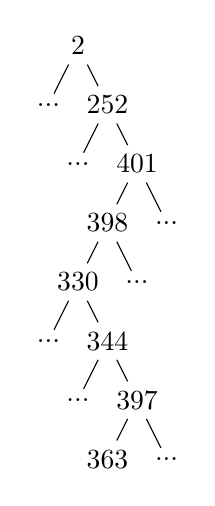
\begin{tikzpicture}[scale=0.5]

\node {2}
	child{node{...}}
	child{ node{252}
		child{node{...}}
		child{node {401}
			child{node{398}
				child{node{330}
					child{node{...}}
					child{node{344}
						child{node{...}}
						child{node{397}
							child{node{363}}
							child{node{...}}}}}
				child{node{...}}}
			child{node{...}}}};
\end{tikzpicture}

\begin{center}
\small
\hspace*{-3cm}
\begin{tabular}{@{} c c l c c @{}}
\toprule
\textbf{Schritt} & \textbf{Aktueller Knoten} & \textbf{Vergleich mit Ziel 363} & \textbf{Nächster Schritt} & \textbf{Intervall für nächsten Knoten} \\
\midrule
1 & 2   & \( 363 > 2 \Rightarrow \) rechts & 252 & \([3, 1000]\) \\
2 & 252 & \( 363 > 252 \Rightarrow \) rechts & 401 & \([253, 1000]\) \\
3 & 401 & \( 363 < 401 \Rightarrow \) links & 398 & \([253, 400]\) \\
4 & 398 & \( 363 < 398 \Rightarrow \) links & 330 & \([253, 397]\) \\
5 & 330 & \( 363 > 330 \Rightarrow \) rechts & 344 & \([331, 397]\) \\
6 & 344 & \( 363 > 344 \Rightarrow \) rechts & 397 & \([345, 397]\) \\
7 & 397 & \( 363 < 397 \Rightarrow \) links & 363 & \([345, 396]\) \\
8 & 363 & Ziel erreicht & — & — \\
\bottomrule
\end{tabular}
\end{center}

\end{answer}

\item \textbf{924, 220, 911, 244, 898, 258, 362, 363.}

\begin{answer}
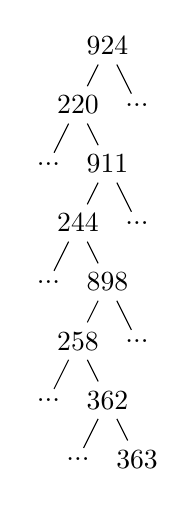
\begin{tikzpicture}[scale=0.5]
\node{924}
	child{node{220}
		child{node{...}}
		child{node{911}
			child{node{244}
				child{node{...}}
				child{node{898}
					child{node{258}
						child{node{...}}
						child{node{362}
							child{node{...}}
							child{node{363}}}}
					child{node{...}}}}
			child{node{...}}}}
	child{node{...}};
\end{tikzpicture}

\begin{center}
\small
\hspace*{-3cm}
\begin{tabular}{@{} c c l c c @{}}
\toprule
\textbf{Schritt} & \textbf{Aktueller Knoten} & \textbf{Vergleich mit Ziel 363} & \textbf{Nächster Schritt} & \textbf{Intervall für nächsten Knoten} \\
\midrule
1 & 924 & \( 363 < 924 \Rightarrow \) links & 220 & \([1, 923]\) \\
2 & 220 & \( 363 > 220 \Rightarrow \) rechts & 911 & \([221, 923]\) \\
3 & 911 & \( 363 < 911 \Rightarrow \) links & 244 & \([221, 910]\) \\
4 & 244 & \( 363 > 244 \Rightarrow \) rechts & 898 & \([245, 910]\) \\
5 & 898 & \( 363 < 898 \Rightarrow \) links & 258 & \([245, 897]\) \\
6 & 258 & \( 363 > 258 \Rightarrow \) rechts & 362 & \([259, 897]\) \\
7 & 362 & \( 363 > 362 \Rightarrow \) rechts & 363 & \([363, 897]\) \\
8 & 363 & Ziel erreicht & — & — \\
\bottomrule
\end{tabular}
\end{center}

\end{answer}


\item \textbf{925, 202, 911, 240, 912, 245, 363.}

\begin{answer}
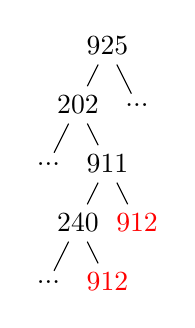
\begin{tikzpicture}[scale=0.5]
\node{925}
	child{node{202}
		child{node{...}}
		child{node{911}
			child{node{240}
				child{node{...}}
				child{node{\textcolor{red}{912}}}}
			child{node{\textcolor{red}{912}}}}}
	child{node{...}};
\end{tikzpicture}

\begin{center}
\small
\hspace*{-3cm}
\begin{tabular}{@{} c c l c c @{}}
\toprule
\textbf{Schritt} & \textbf{Aktueller Knoten} & \textbf{Vergleich mit Ziel 363} & \textbf{Nächster Schritt} & \textbf{Intervall für nächsten Knoten} \\
\midrule
1 & 925 & \( 363 < 925 \Rightarrow \) links & 202 & \([1, 924]\) \\
2 & 202 & \( 363 > 202 \Rightarrow \) rechts & 911 & \([203, 924]\) \\
3 & 911 & \( 363 < 911 \Rightarrow \) links & 240 & \([203, 910]\) \\
4 & 240 & \( 363 > 240 \Rightarrow \) rechts & 912 & \([241, 910]\) \\
5 & 912 & \( 363 < 912 \Rightarrow \) links & & \textcolor{red}{\( 912 > [910] \Rightarrow \) Fehler} \\
\bottomrule
\end{tabular}
\end{center}

\begin{itemize}
	\item Der Knoten 912 liegt nicht mehr im Intervall von [241,910] und somit ist der Knoten nicht in der \textbf{Schlüsselfolge}.
\end{itemize}
\end{answer}

\item \textbf{2, 399, 387, 219, 266, 382, 381, 278, 363.}

\begin{answer}
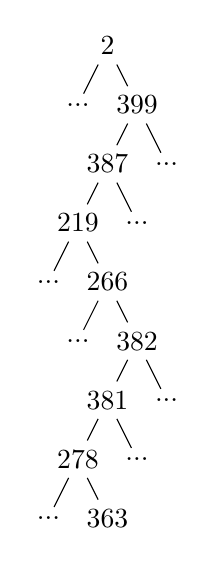
\begin{tikzpicture}[scale=0.5]
\node{2}
	child{node{...}}
	child{node{399}
		child{node{387}
			child{node{219}
				child{node{...}}
				child{node{266}
					child{node{...}}
					child{node{382}
						child{node{381}
							child{node{278}
								child{node{...}}
								child{node{363}}}
							child{node{...}}}
						child{node{...}}}}}
			child{node{...}}}
		child{node{...}}};
\end{tikzpicture}

\begin{center}
\small
\hspace*{-3cm}
\begin{tabular}{@{} c c l c c @{}}
\toprule
\textbf{Schritt} & \textbf{Aktueller Knoten} & \textbf{Vergleich mit Ziel 363} & \textbf{Nächster Schritt} & \textbf{Intervall für nächsten Knoten} \\
\midrule
1 & 2 & \( 363 > 2 \Rightarrow \) rechts & 399 & \([3, 1000]\) \\
2 & 399 & \( 363 < 399 \Rightarrow \) links & 387 & \([3, 398]\) \\
3 & 387 & \( 363 < 387 \Rightarrow \) links & 219 & \([3, 386]\) \\
4 & 219 & \( 363 > 219 \Rightarrow \) rechts & 266 & \([220, 386]\) \\
5 & 266 & \( 363 > 266 \Rightarrow \) rechts & 382 & \([267, 386]\) \\
6 & 382 & \( 363 < 382 \Rightarrow \) links & 381 & \([267, 381]\) \\
7 & 381 & \( 363 < 381 \Rightarrow \) links & 278 & \([267, 380]\) \\
8 & 278 & \( 363 > 278 \Rightarrow \) rechts & 363 & \([279, 380]\) \\
9 & 363 & Ziel Erreicht! & - & - \\
\bottomrule
\end{tabular}
\end{center}

\end{answer}

\item \textbf{935, 278, 347, 621, 299, 392, 358, 363.}

\begin{answer}
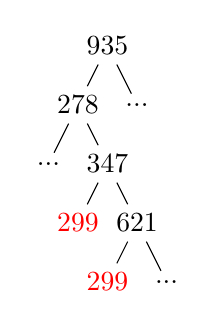
\begin{tikzpicture}[scale=0.5]
\node{935}
	child{node{278}
		child{node{...}}
		child{node{347}
			child{node{\textcolor{red}{299}}}
			child{node{621}
				child{node{\textcolor{red}{299}}}
				child{node{...}}}}}
	child{node{...}};
\end{tikzpicture}

\begin{center}
\small
\hspace*{-3cm}
\begin{tabular}{@{} c c l c c @{}}
\toprule
\textbf{Schritt} & \textbf{Aktueller Knoten} & \textbf{Vergleich mit Ziel 363} & \textbf{Nächster Schritt} & \textbf{Intervall für nächsten Knoten} \\
\midrule
1 & 935 & \( 363 < 935 \Rightarrow \) links & 278 & \([1, 934]\) \\
2 & 278 & \( 363 > 278 \Rightarrow \) rechts & 347 & \([279, 934]\) \\
3 & 347 & \( 363 > 347 \Rightarrow \) rechts & 621 & \([348, 934]\) \\
4 & 621 & \( 363 < 621 \Rightarrow \) links & 299 & \([348, 620]\) \\
5 & 299 & \( 363 > 299 \Rightarrow \) rechts & & \textcolor{red}{\( 299 < [348] \Rightarrow \) Fehler} \\
\bottomrule
\end{tabular}
\end{center}

\begin{itemize}
	\item Der Knoten 299 liegt nicht mehr im Intervall von [348,620] und somit ist der Knoten nicht in der \textbf{Schlüsselfolge}.
\end{itemize}

\end{answer}

\end{enumerate}

\item Sei T ein binärer Baum mit n Knoten, und sei K eine total geordnete Menge
von n Schlüsseln. Zeigen Sie, dass es genau eine Möglichkeit gibt, die Schlüssel
aus K auf die Knoten von T zu verteilen, so dass die binäre Suchbaumeigen-
schaft erfüllt ist.
\end{enumerate}


\pbitem{AVL-Bäume}
\begin{enumerate}
\item Fügen Sie die Schlüssel A, L, G, O, D, T, S, X, Y, Z in dieser Reihenfolge in
einen anfangs leeren AVL-Baum ein. Löschen Sie sodann die Schlüssel Z, A,
L. Zeichnen Sie den Baum nach jedem Einfüge- und Löschvorgang, und zeigen
Sie die Rotationen, welche durchgeführt werden. Annotieren Sie dabei auch
die Knoten mit ihrer jeweiligen Höhe.

\item Beweisen Sie: Beim Einfügen in einen AVL-Baum wird höchstens eine (Einfach-
oder Doppel-)Rotation ausgeführt. Gilt das auch beim Löschen (Begründung)?
\end{enumerate}


	
	
	
\end{problemlist}

%Quellen Reference
%\newpage
%\printbibliography

\end{document}